\documentclass[UTF8]{ctexart}

%固定图片位置
\usepackage{float}

\usepackage{tikz,mathpazo}
\usetikzlibrary{shapes.geometric, arrows}
\usetikzlibrary{calc}


\usepackage{listings}
%插入代码的配置
\definecolor{CPPLight}  {HTML} {686868}
\definecolor{CPPSteel}  {HTML} {888888}
\definecolor{CPPDark}   {HTML} {262626}
\definecolor{CPPBlue}   {HTML} {4172A3}
\definecolor{CPPGreen}  {HTML} {487818}
\definecolor{CPPBrown}  {HTML} {A07040}
\definecolor{CPPRed}    {HTML} {AD4D3A}
\definecolor{CPPViolet} {HTML} {7040A0}
\definecolor{CPPGray}  {HTML} {B8B8B8}
\lstset{
	language=Python,                                     % 设置语言
    columns=fixed,    
    breaklines = true,   
    basicstyle=\small ,
    numbers=left,                                        % 在左侧显示行号
    %frame=none,                                          % 不显示背景边框
    backgroundcolor=\color[RGB]{245,245,244},            % 设定背景颜色
    keywordstyle=\color[RGB]{40,40,255},                 % 设定关键字颜色
    numberstyle=\tiny\color{darkgray},           % 设定行号格式
    %commentstyle=\it\color[RGB]{0,96,96},                % 设置代码注释的格式
    stringstyle=\rmfamily\slshape\color[RGB]{128,0,0},   % 设置字符串格式
    showstringspaces=false,                              % 不显示字符串中的空格                           
    %morekeywords={True,alignas,continute,friend,register,true,alignof,decltype,goto,
    %reinterpret_cast,try,asm,defult,if,return,typedef,auto,delete,inline,short,
    %typeid,bool,do,int,signed,typename,break,double,long,sizeof,union,case,
    %dynamic_cast,mutable,static,unsigned,catch,else,namespace,static_assert,using,
    %char,enum,new,static_cast,virtual,char16_t,char32_t,explict,noexcept,struct,
    %void,export,nullptr,switch,volatile,class,extern,operator,template,wchar_t,
    %const,false,private,this,while,constexpr,float,protected,thread_local,
    %const_cast,for,public,throw,std,rand},
    emph={access,and,break,class,continue,def,del,elif ,else,%
	except,exec,finally,for,from,global,if,import,in,i s,%
	lambda,not,or,pass,print,raise,return,try,while},
    emphstyle=\color{CPPViolet}, 
    emph={[2]True, False, None, self},
	emphstyle=[2]\color{green},
	emph={[3]from, import, as},
	emphstyle=[3]\color{blue},
	upquote=true,
	morecomment=[s]{"""}{"""},
	commentstyle=\color{orange}\slshape,
	emph={[4]1, 2, 3, 4, 5, 6, 7, 8, 9, 0},
	emphstyle=[4]\color{red},
	emph={[5]numpy, np, plt},
	emphstyle=[5]\color{red},
	literate=*{:}{{\textcolor{blue}:}}{1}%
	{=}{{\textcolor{blue}=}}{1}%
	{-}{{\textcolor{blue}-}}{1}%
	{+}{{\textcolor{blue}+}}{1}%
	{*}{{\textcolor{blue}*}}{1}%
	{!}{{\textcolor{blue}!}}{1}%
	{(}{{\textcolor{blue}(}}{1}%
	{)}{{\textcolor{blue})}}{1}%
	{[}{{\textcolor{blue}[}}{1}%
	{]}{{\textcolor{blue}]}}{1}%
	{<}{{\textcolor{blue}<}}{1}%
	{>}{{\textcolor{blue}>}}{1},%
	framexleftmargin=0.1mm, framextopmargin=0.1mm, frame=shadowbox, rulesepcolor=\color{black},
}



\usepackage{geometry}
\geometry{left=2cm, right=2cm, top=1.2cm, bottom=1.2cm}

%得到引用的标题内容
\usepackage{nameref} 

%添加首行缩进,两个字符
\usepackage{indentfirst}
\setlength{\parindent}{2em}

%多行公式一个编号
\usepackage{amsmath}

%文献引用,标准类型为plain
%\usepackage[hyperref=true,backend=biber,sorting=none,backref=true]{biblatex}
%\addbibresource{ref.bib}
\bibliographystyle{plain}
\usepackage{cite}

\pagestyle{plain}

%跨页表格
\usepackage{multirow}
\usepackage{longtable,booktabs}
\usepackage{supertabular}
\usepackage{makecell}

%调整itemize等的间距
\usepackage{enumitem}


\usepackage{graphicx}

%超链接
\usepackage[linkcolor=yellow,citecolor=red,backref=page]{hyperref}
\hypersetup{
bookmarks=true,
colorlinks=true,
linkcolor=black
}

%引入了一些改进的数学环境,如align
\usepackage{amsmath}

\title{数据结构:祖玛}
\author{姓名:鲁国锐 \protect\newline
\and 学号:17020021031 \\
\and 专业:电子信息科学与技术}


\begin{document}
	\maketitle
	\renewcommand{\contentsname}{Contents}
	\tableofcontents
	\newpage
	
	\hypersetup{
	bookmarks=true,
	colorlinks=true,
	linkcolor=red,
	urlcolor=blue
	}
	\section{问题分析}
	\subsection{题目描述}
	\indent 自己编写$list$ $ADT$,调试并完成下面内容。注:本次作业不允许使用$c++$标准模版库。
	\begin{itemize}[leftmargin=60pt]
	
	\item 任务一:
	\begin{itemize}
		\item[$\circ$] 实现$PrintLots(L,P)$,并分析运行时间。
		\item[$\circ$] 有两个链表$L$和$P$, 他们包含以升序排列的整数。操作$PrintLots(L,P)$将打印$L$中那些由$P$所指定位置上的元素。如:$P={1,3,4,6}$, 则,$L$中第$1$,第$3$,第$4$,第$6$个元素被打印出来。
	\end{itemize}
		

	\item 任务二:懒惰删除
	\begin{itemize}
		\item[$\circ$] 列出懒惰删除的优点和缺点
		\item[$\circ$] 编写实现
		
		不同于我们已经给出的删除方法,另一种是使用懒惰删除($lazy\ deletion$)。为了删除一个元素,我们只标记上该元素被删除。表中被删除和非被删除元素的个数作为数据结构的一部分被保留。如果被删除元素和非被删除元素一样多,我们遍历整个表,对所有被标记的节点执行标准的删除算法。
	\end{itemize}			
	\end{itemize}
	

	\subsection{问题分析}
	\indent 根据题目,我们需要解决的问题有:
	\begin{enumerate}[leftmargin=50pt]

	\item 编写$Node$和$List$类,包括实现$List$中一系列必须的成员函数,如:构造函数、析构函数、$insert$函数、$remove$函数等(见\ref{desigh_class}节);
	\item 设计输入输出流程(见\ref{design_input_and_output}节);
	\item 实现$PrintLots$函数(见\ref{PrintLots}节)和$lazy\ deletion$函数(见\ref{lazy_del}节)及其相关的部分函数;
	\item 分析$PrintLots$的时间复杂度(见\ref{time_of_PrintLots}节);
	\item 分析懒惰删除的有点和缺点(见\ref{adv_and_disadv_of_lazy_deletion}节)。
	\end{enumerate}
	

	
	\section{解决方案}
		\subsection{编写$Node$类和$List$类}\label{desigh_class}
			\indent 我们首先要写$Node$类,它的属性包括值$val$、指向前驱的指针$pred$、指向后继的指针$succ$以及在本题中需额外设置的一个属性$deleted$,用以表示该节点是否被标记为删除。其构造函数相对简单,在此不做赘述。
			
			\indent 接下来是$List$类,它的属性包括头指针$header$、尾指针$trailer$、长度$\_size$(不包括头指针和尾指针)和被标记为删除的元素个数$\_delNum$。至于其成员函数,由于数量较多,我们只用一表格列出,并做简要说明。
			\begin{center}
			\begin{longtable}[H]{|c|c|c|c|}
            \caption{$List$成员函数}
            \label{functions}
			\\
			\hline
			\textbf{函数名}&\textbf{输入}&\textbf{输出}&\textbf{说明} \\
			\hline
			\endfirsthead
			
			\hline
			\textbf{函数名}&\textbf{输入}&\textbf{输出}&\textbf{说明} \\
			\hline
			\endhead
			
			\hline
			\multicolumn{4}{|c|}{\textsl{下页继续}} \\
			\hline
			\endfoot
			
			\hline
			\endlastfoot
			
			\hline
			构造函数&无&无&初始化整个链表,建立头结点和尾节点 \\			
				
			\hline
			析构函数&无&无&删除链表,释放内存 \\			
			
			\hline
			$insert$&指针$r$,值$e$&该节点的指针&在$r$所指向的节点之前插入一个节点 \\
			
			\hline
			$push\_back$&值$e$&无&在尾节点之前插入一个结点 \\
			\hline
			
			$remove$&指针$r$&被删除节点下一个节点的指针&\makecell{删除$r$指向的节点} \\
			\hline
			
			$clear$&无&被删除元素的个数&清空链表(不包括头结点和尾节点)\\
			\hline
			
			$clear\_mark$&无&无&\makecell{调用$remove$函数清除所有被标记为\\已删除的节点} \\
			\hline
			
			$lazeDel$&指针$r$&被删除元素的值&\makecell{用懒惰删除的方式删除$r$指向的节点} \\
			\hline
			
			$getP$&序号(从$1$开始计数)&指向序号所对应的节点的指针&将输入的序号转换为指针,方便后续的操作 \\
			\hline 
			
			$print$&无&无&\makecell{输出链表中所有节点的值\\(不包括头结点和尾节点)} \\
			\hline
			
			$getHeader$&无&头指针&返回头指针 \\
			\hline
			
			$getTrailer$&无&尾指针&返回尾指针 \\
			\hline 
			
			$size$&无&\makecell{链表长度\\(不包括头结点和尾节点)}&返回链表长度(不包括头结点和尾节点) \\
			\hline

			\end{longtable}			
			\end{center}
		
		
		\subsection{设计输入输出流程}\label{design_input_and_output}
		\indent 我们首先输入链表$L$各节点的值,这些值以空格分隔,以回车结束。然后通过三条指令来控制这个程序的流程:
			\begin{itemize}[leftmargin=50pt]
			\item $delete$:执行懒惰删除操作,后跟一数字表示要删除节点的序号;
			\item $PrintLots$:调用$PrintLots$函数,后跟一组以空格分隔的数字,表示链表$P$中各节点的元素;
			\item $end$:结束整个程序。
			\end{itemize}
			
		\indent 每次执行完$delete$或$PrintsLots$后,把$L$中各节点的值输出一遍。其中在执行$PrintLots$时还会把$P$以及$L$中对应于$P$所表示的序号的节点值输出一遍,分别以“$P:$”和“$L:$”开头。
		
		\subsection{实现$PrintLots$函数}\label{PrintLots}
		\indent 有了表\ref{functions}中的各个函数,我们实现$PrintLots$就会轻松不少。
		
		\indent 首先我们要检查$L$是否为空,若为空则直接结束函数的调用。若不为空,我们开始执行输出操作。这里定义了两个指针$pl$和$pp$,分别初始化为指向$L$的头节点和$P$的第一个节点。同时为了避免在得到$P$中节点的值后要从头开始遍历$L$,我们还需定义两个整型变量$pre$和$offset$。其中$pre$中记录的是$P$中前一个节点的值,而$offset$中记录的则是$pl$需要向后移动的位数。每次我们令$pp$向后移动一位,然后用$pp$指向的节点中的值减去$pre$,所得结果赋给$offset$,然后令$pl$向后移$offset$位,输出其对应节点中的值。
		
		\indent 另外在执行输出操作时我们还要不断检查$pl$是否越界。如果发现$pl$指向了尾节点,立马抛出异常并结束整个函数。
		\subsection{实现$lazy\ deletion$函数}\label{lazy_del}
		\indent 这个函数实现起来相对简单。我们只需要把传入指针对应的节点中$deleted$属性置为$true$即可。同时还要将链表中的$\_delNum$加一。然后判断$\frac{\_size}{2} \leq \_delNum$是否成立。若成立,则执行$clear_mark$函数,将链表中所有$deleted$为$true$的节点删除,并把$\_delNum$值$0$。
	\section{算法设计}
	见下页图\ref{PrintsLots_and_lazeDel}、图\ref{main}。

\begin{figure}[H]
	\centering 
	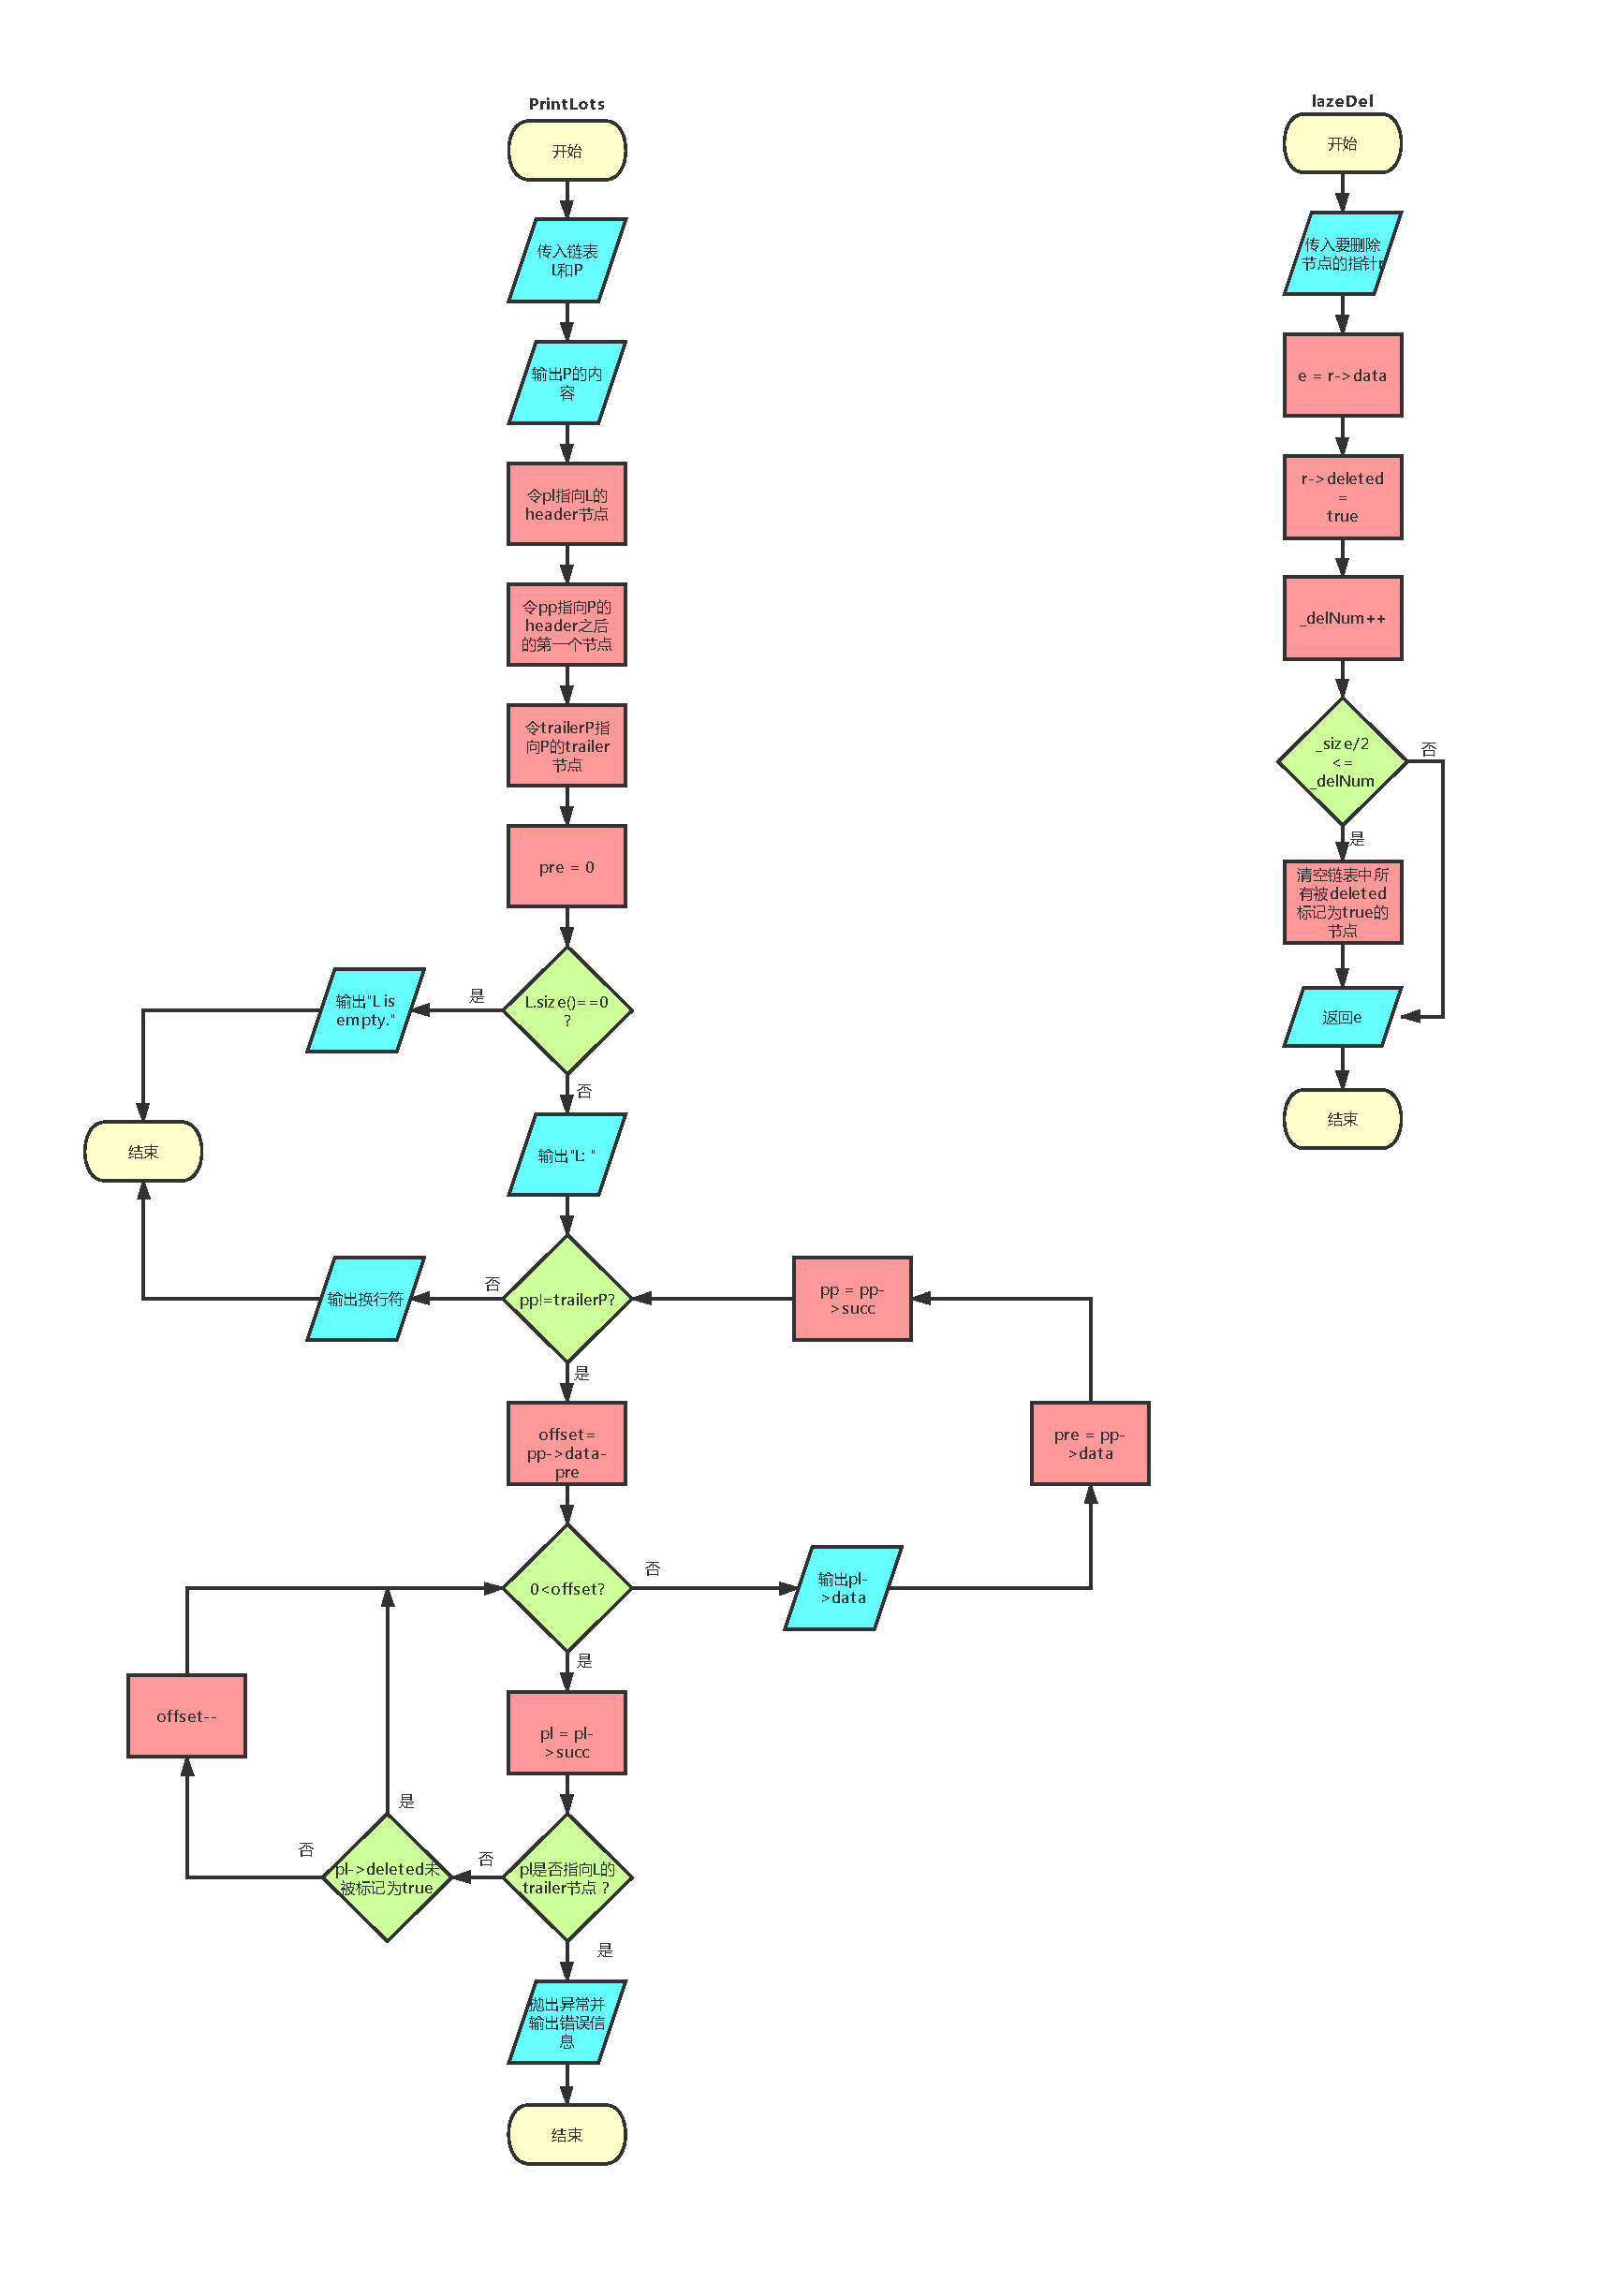
\includegraphics[width=20cm, height=25cm]{list_ADT.pdf} 
	\caption{$PrintLots$和$lazeDel$函数流程图} 
	\label{PrintsLots_and_lazeDel}
\end{figure}



\begin{figure}[H]
	\centering 
	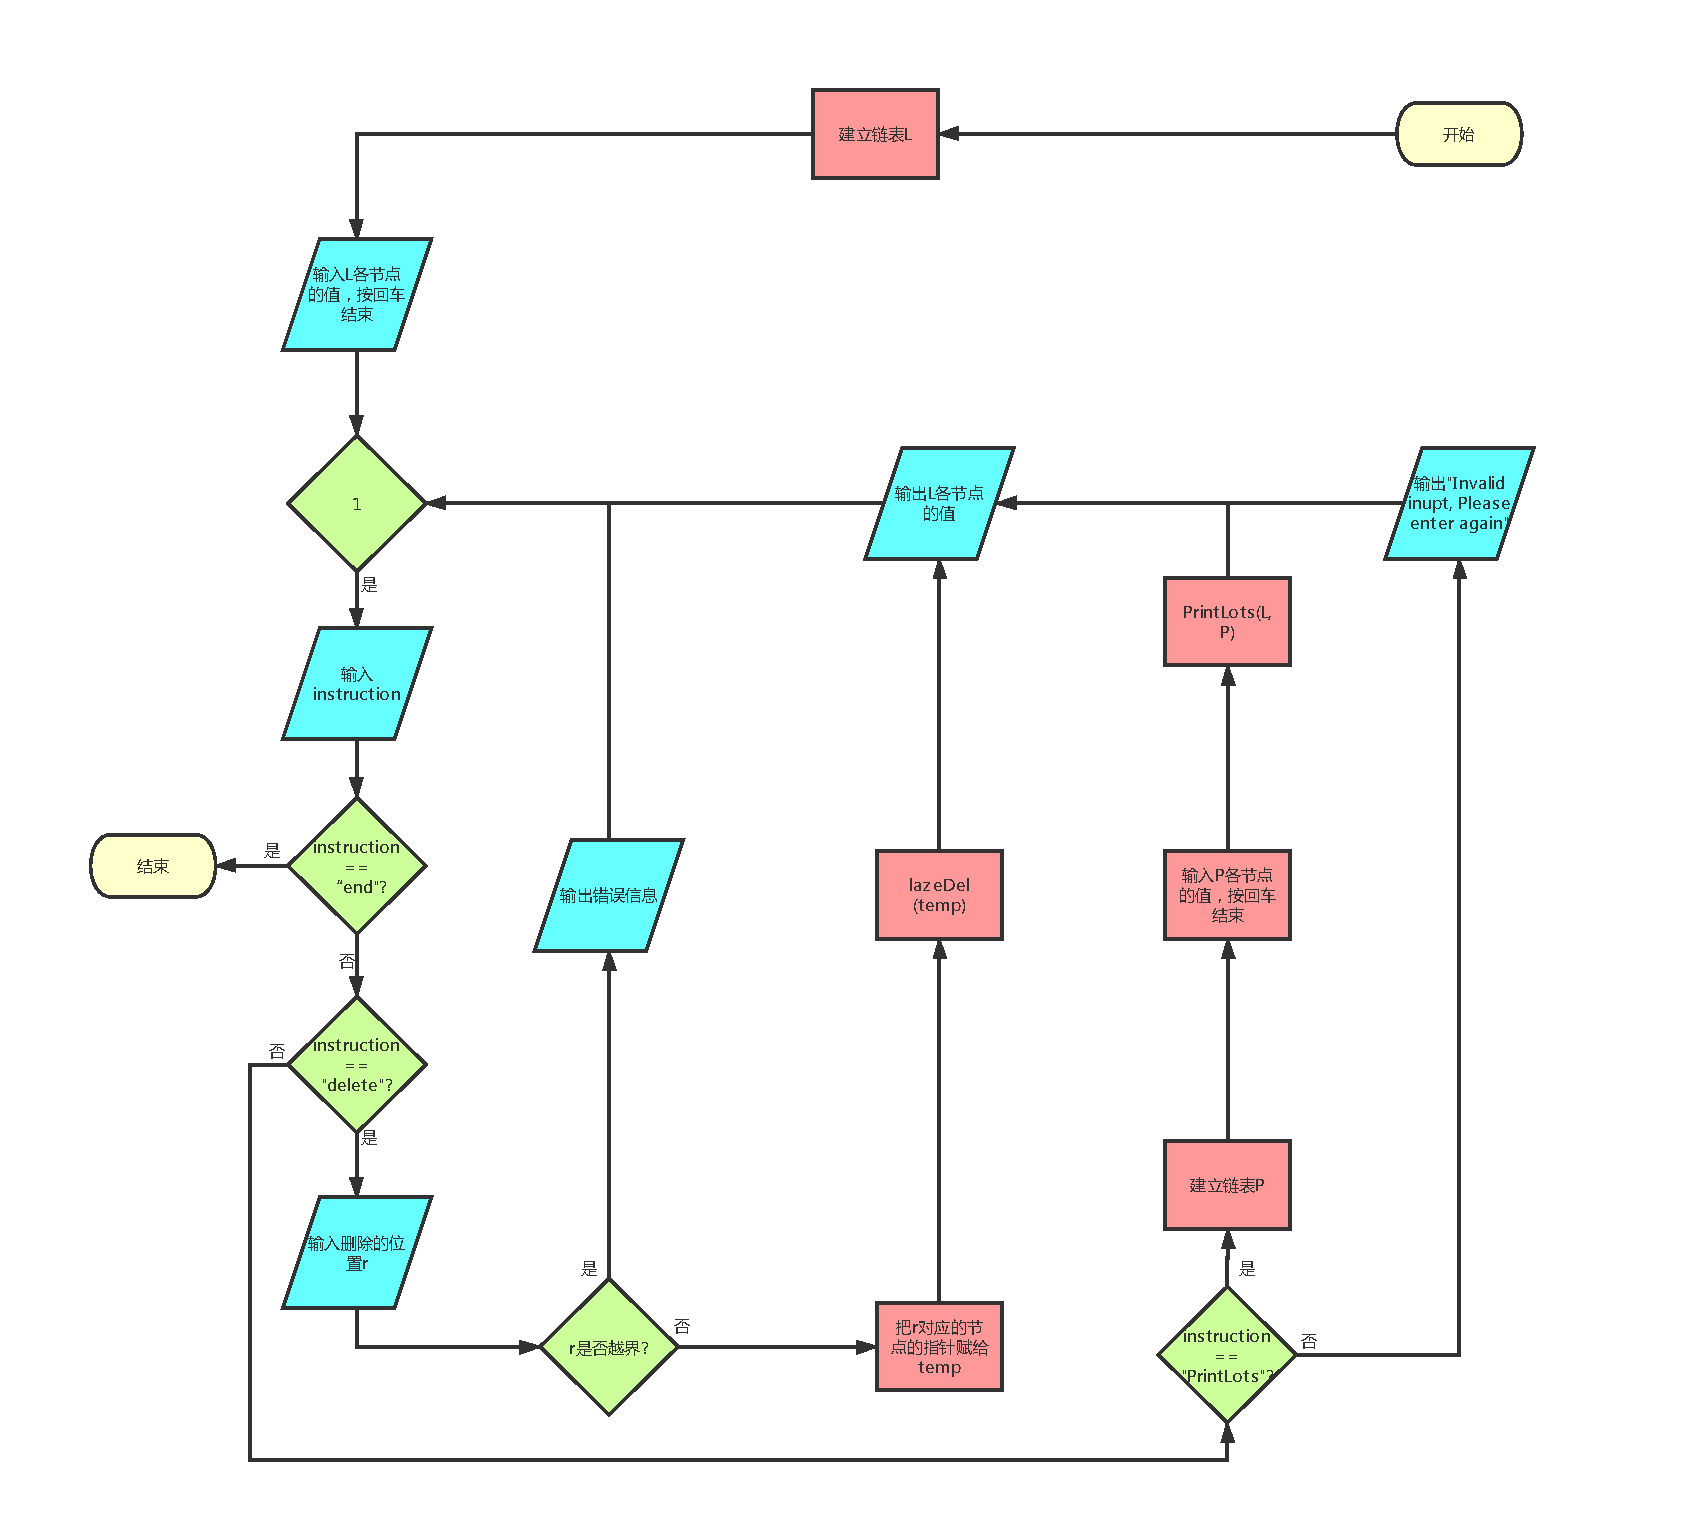
\includegraphics[width=20cm, height=23cm]{list_ADT_main.pdf} 
	\caption{$main$函数流程图} 
	\label{main}
\end{figure}
\newpage



	\section{编程实现}

	\begin{lstlisting}[language=C++,caption={list\_ADT代码},label={vec_code}]
#include<iostream>
#include<exception>
#include<stdexcept>
using namespace std;

template <typename T> 
class Node
{
    public:
        // member variables
        T data;
        Node<T>* pred;
        Node<T>* succ;
        bool deleted;
        // constructors
        Node() : data(0), pred(NULL), succ(NULL){}
        Node(T e, Node<T>* p=NULL, Node<T>* s=NULL) : data(e), pred(p), succ(s), deleted(false) {}
        // operation interface
        //Node<T>* insertAsPred(T const& e);
        //Node<T>* insertAsSucc(T const& e);
};


template <typename T> 
class List
{
    private:
        int _size;
        Node<T>* header;
        Node<T>* trailer;
        int _delNum;
    public:
        // constructors
        List();

        // destructor
        ~List();

        // operation interfaces
        Node<T>* insert(Node<T>* r, T const& e);// insert as pred
        void push_back(T e) {insert(trailer, e);}
        Node<T>* remove(Node<T>* r);
        int clear();
        void clear_mark();
        T lazeDel(Node<T>* r);
        Node<T>* getP(int r);
        void print();
        Node<T>* getHeader() {return header;}
        Node<T>* getTrailer() {return trailer;}
        int size() {return _size;}
};
// implement the functions of the List
template <typename T>
List<T>::List()
{
    header = new Node<T>;
    trailer = new Node<T>;
    header->succ = trailer;
    header->pred = NULL;
    trailer->pred = header;
    trailer->succ = NULL;
    _size = 0;
    _delNum = 0;
}

template <typename T>
Node<T>* List<T>::insert(Node<T>* r, T const& e)
{
    // insert as pred
    Node<T>* x = new Node<T>(e, r->pred, r);
    r->pred->succ = x;
    r->pred = x;
    _size++;
    return x;
}

template <typename T>
Node<T>* List<T>::remove(Node<T>* r)
{
    r->pred->succ = r->succ;
    r->succ->pred = r->pred;
    Node<T>* p = r->succ;
    delete r;
    _size--;
    if (r->deleted) _delNum--;
    return p;
}

template <typename T>
int List<T>::clear()
{
    int oldSize = _size;
    while(0 < _size)
        remove(header->succ);
    return oldSize;
}

template <typename T>
void List<T>::clear_mark()
{
    Node<T>* p = header->succ;
    while (p != trailer)
    {
        if (p->deleted)
            p = remove(p);
        else
            p = p->succ;
    }
    _delNum = 0;
    cout << "remove all nodes marked." << endl;
}

template <typename T>
List<T>::~List()
{
    clear();
    delete header;
    delete trailer;
}

template <typename T>
T List<T>::lazeDel(Node<T>* r)
{
    T e = r->data;
    r->deleted = true;
    _delNum++;
    if (_size/2 <= _delNum)
        clear_mark();
    return e;
}

template <typename T>
Node<T>* List<T>::getP(int r)
{
    Node<T>* p = header;
    while (0 < r)
    {
        p = p->succ;
        if (!p->deleted)
            r--;
        if (p == trailer)
            throw out_of_range("Overflow!");

    }

    return p;
}

template <typename T>
void List<T>::print()
{
    if (_size == 0)
    {
        cout << "The list is empty." << endl;
        return;
    }
    Node<T>* p = header;
    while ((p = p->succ) != trailer)
        if (!p->deleted)
            cout << p->data << " ";
    cout << endl;
}




// implement PrintLots
template <typename T>
void PrintLots(List<T>& L, List<T>& P)
{
    cout << "P: ";
    P.print();
    // pl points to the header of L 
    // and pp points to the first element of P
    Node<T>* pl = L.getP(0);
    Node<T>* pp = P.getP(1);
    Node<T>* trailerP = P.getTrailer();
    int pre = 0;
    if (!L.size())
    {
        cout << "L is empty." << endl;
        return;
    }
    cout << "L: ";
    while (pp != trailerP)
    {
        int offset = pp->data - pre;
        while (0 < offset)
        {
            pl = pl->succ;
            try
            {
                if (pl == L.getTrailer())
                    throw out_of_range("Overflow!");
            }catch(out_of_range &e)
            {
                cerr << endl << "Index " << pp->data <<" is out of range. " << e.what() << endl;
                return;
            }
            if (!pl->deleted)
                offset--;
        }
        cout << pl->data << " ";
        pre = pp->data;
        pp = pp->succ;
    }
    cout << endl;
}




int main()
{
    cout << "姓名:鲁国锐" << endl;
    cout << "学号:17020021031" << endl;
    cout << endl;
    cout << "instructions:" << endl;
    cout << "delete: 后跟一数字,执行懒惰删除操作" << endl;
    cout << "PrintLots: 后跟若干数字,务以空格分隔,以回车结束输入,为链表P的节点值,执行PrintLots操作" << endl;
    cout << "end: 结束程序" << endl;

    cout << endl << "请输入L中各节点的值,务必以空格分隔,以回车结束输入:" << endl;

    List<int> L;

    while (1)
    {
        int data;
        char c;
        cin >> data;
        cin.get(c);
        L.push_back(data);
        if (c == '\n')
            break;
    }
  
    while(1)
    {
        string instruction;
        cin >> instruction;
        if (instruction == "end")
            break;
        else if (instruction == "delete")
        {
            int r;
            cin >> r;
            Node<int>* temp;
            try
            {
                temp = L.getP(r);
            }catch(out_of_range &e)
            {
                cerr << "Index " << r << " is out of range. " << e.what() << endl;
                continue;
            }
            L.lazeDel(temp);
        }
        else if (instruction == "PrintLots")
        {
            List<int> P;
            while (1)
            {
                int data;
                char c;
                cin >> data;
                cin.get(c);
                P.push_back(data);
                if (c == '\n')
                    break;
            }
            PrintLots(L, P);
        }
        else
        {
            cout << "Invalide input, please enter again." << endl;
            continue;
        }
        

        L.print();
    }
}
	\end{lstlisting}
	
	\section{结果分析}
	\subsection{结果展示}
	\newpage
\begin{figure}[H]
	\centering 
	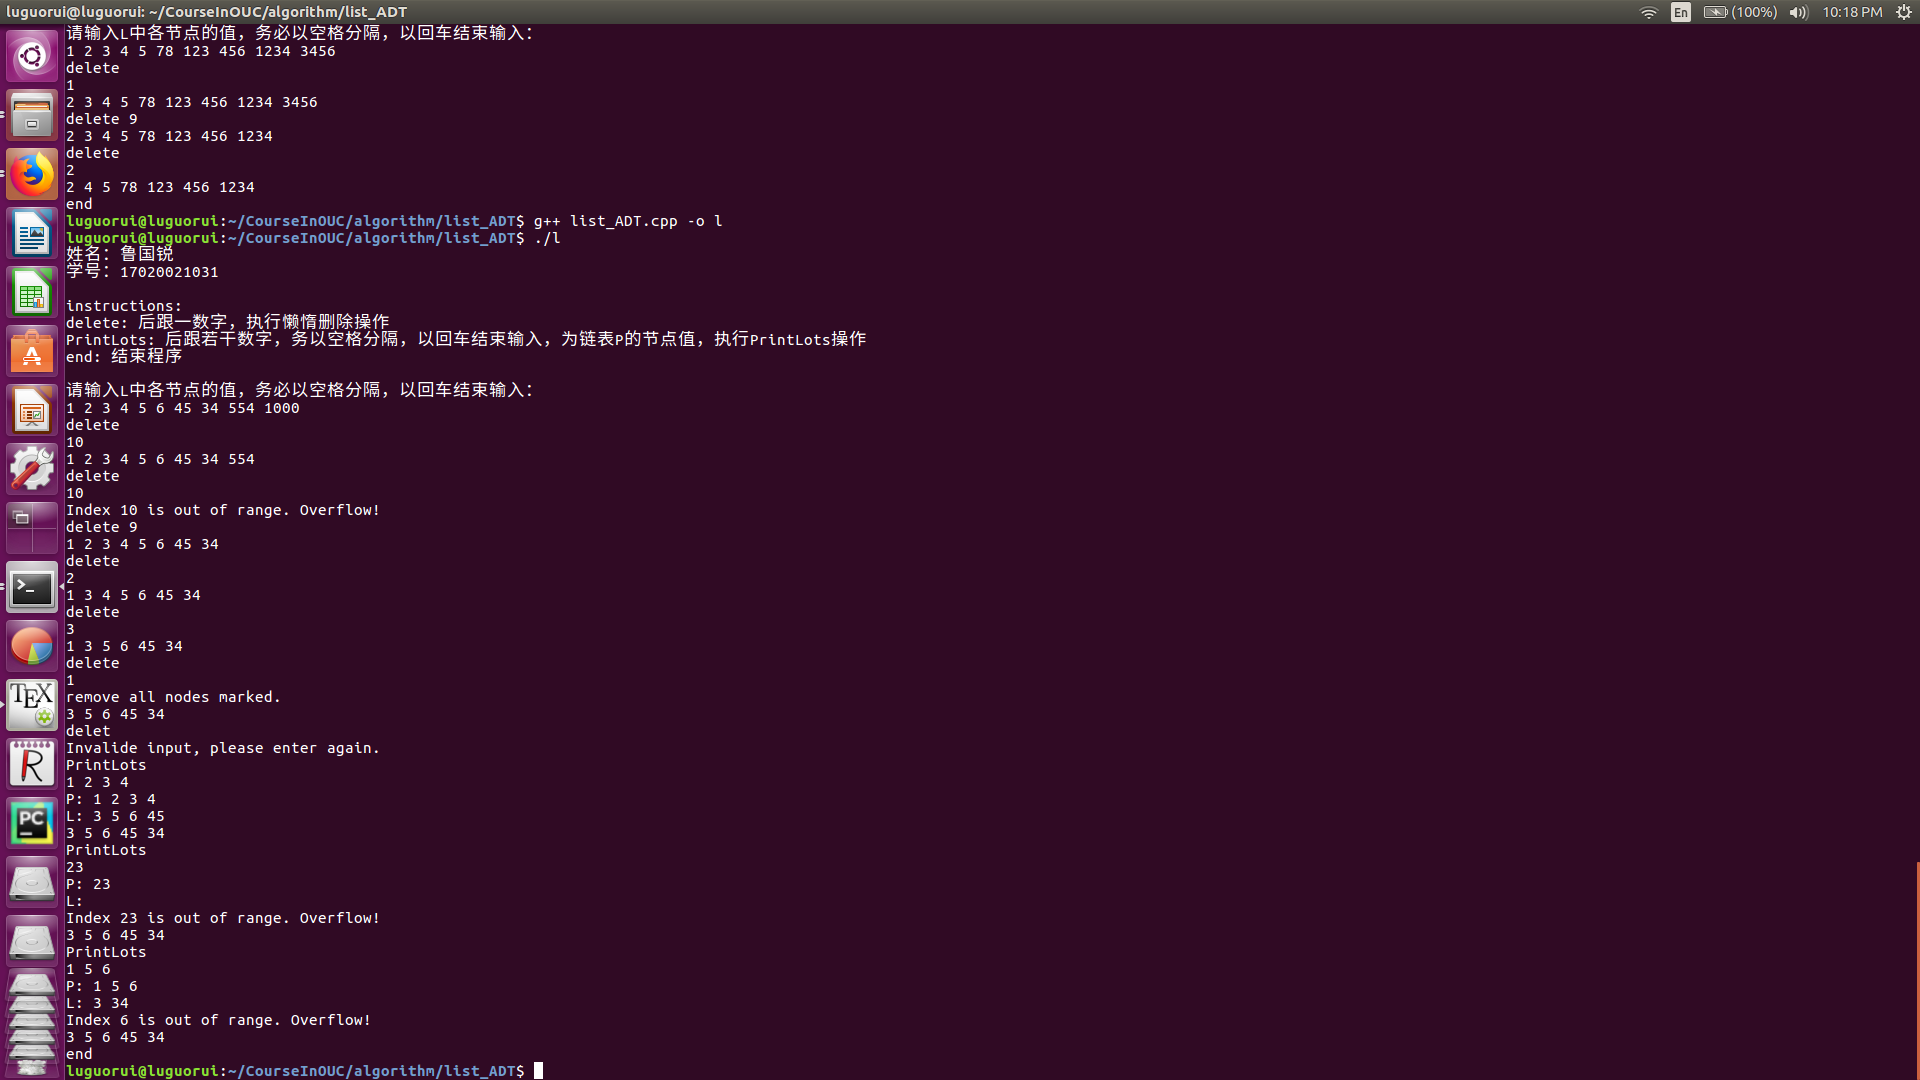
\includegraphics[width=18cm, height=23cm]{list_res.png} 
	\caption{结果} 
	\label{res}
\end{figure}


	\subsection{$PrintLots$运行时间}\label{time_of_PrintLots}
	\indent 由于我们在执行输出操作时引入$pre$和$offset$两个变量从而避免了对$L$的重复遍历。因此,即使在最坏情况下,即需要输出$L$中的最后一个元素时,我们也只需令$pl$向后移动$L.\_size$次,所需时间与$L$的长度成正比。故其时间复杂度为$O(N)$。
	
	\subsection{懒惰删除的优点和缺点}\label{adv_and_disadv_of_lazy_deletion}
	\indent 懒惰删除的优点:
	\begin{itemize}[leftmargin=50pt]
	\item 减少删除节点时所需的时间;
	\item 避免频繁地对内存进行操作;
	\item 简化代码复杂程度;
	\item 在对被删除位置进行插入时\textbf{可能}会减少时间。
	\end{itemize}
	
	\indent 懒惰删除的缺点:
	\begin{itemize}[leftmargin=50pt]
	\item 会占用更多的空间;
	\item 由于在链表中由于并没有真正删除节点,所以会增减遍历链表所需的时间;
	\end{itemize}
	\section{总结体会}
	\indent 在完成这次作业的过程中,由于一开始没有加入检查指针是否越界的代码,导致在调试过程中因指针越界使得电脑死机了,从而不得不强制关机重启。这次的教训让我更深刻地明白了检查指针越界的重要性,同时还促使我去学习了如何在$C++$中捕获异常并输出错误信息。
	\indent 另外还没有完全解决的一点是,因为我不想在输入链表的值之前还要输入长度,所以采取的做法是当检测到输入数字后跟的是回车时就跳出循环。但如果在输入回车之前不小心多输入了空格,
并在输入回车后输入命令,也会使电脑几乎陷入死机状态。我暂时还没想出是什么原因导致的,也没有很好的解决方法。

\bibliography{ref.bib}
\end{document}